\documentclass[12pt,a4paper]{article}
\usepackage[utf8]{vietnam}
\usepackage{amsmath,amssymb}
\usepackage{tabularx}
\usepackage{graphicx}
\usepackage{tikz}
\usetikzlibrary{calc,arrows.meta}
\usepackage{xcolor}
\usepackage{enumitem}
\usepackage{fancyhdr}
\usepackage[top=0.8cm, bottom=0.8cm, left=1.2cm, right=1.2cm]{geometry}
\usepackage[dethi]{ex_test}
\SAOPTN{widthSA=2.6,heightSA=0.62}

\setlength{\headheight}{15pt}
\setlength{\parskip}{0pt}

% Dòng kẻ chấm mờ chuẩn viết tay
\newcommand{\dongke}[1]{%
  \begingroup%
  \setlength{\parskip}{0pt}%
  \baselineskip=18.5pt%
  \vspace{1.0mm}%
  \foreach \i in {1,...,#1}{%
    \noindent{\color{gray!60}\dotfill}\par%
  }%
  \vspace{0.6mm}%
  \endgroup%
}

\pagestyle{fancy}
\fancyhf{}
\rhead{\textit{Môn Toán 7 -- Đề số 10}}
\lhead{\textit{Bộ đề ôn tập Giữa học kì I}}
\cfoot{\thepage}

\begin{document}

% --- KHUNG TIÊU ĐỀ ĐỀ THI ---
\noindent
\begin{tabularx}{\linewidth}{X r}
\textbf{TRƯỜNG THCS: \dotfill} & \textbf{ĐỀ KIỂM TRA ĐỊNH KỲ GIỮA HỌC KỲ I} \\
\textbf{Họ và tên: \dotfill} & \textbf{NĂM HỌC 2026 -- 2027} \\
\textbf{Lớp: \dotfill \quad SBD: \dotfill} & \textbf{Môn: TOÁN 7} \\
& \textit{Thời gian làm bài: 90 phút (không kể thời gian phát đề)}
\end{tabularx}

\vspace{1mm}
\noindent
\begin{tabularx}{\linewidth}{|p{3.5cm}|X|}
\hline
\centering\textbf{Điểm số} & \centering\textbf{Lời nhận xét của thầy cô giáo} \tabularnewline
\rule{0pt}{0.8cm} & \\
\hline
\end{tabularx}

\vspace{1.5mm}
\begin{center}
\textbf{\large ĐỀ SỐ 10}
\end{center}

\noindent\textbf{\large PHẦN I. CÂU TRẮC NGHIỆM NHIỀU PHƯƠNG ÁN LỰA CHỌN (3,0 điểm)}

\textit{Thí sinh trả lời từ câu 1 đến câu 12. Mỗi câu hỏi chỉ chọn một phương án đúng nhất và ghi vào bảng đáp án.}

\vspace{1mm}
\begin{ex}
Số nào dưới đây là số thập phân vô hạn tuần hoàn?
\choice
{$\dfrac{1}{2}$}
{$0{,}123123$}
{\True $0{,}(3)$}
{$0{,}3$}
\end{ex}

\begin{ex}
\immini{
Điểm $A$ trên trục số ở hình bên biểu diễn số hữu tỉ nào?
\choice
{$-\dfrac{2}{3}$}
{$\dfrac{1}{3}$}
{\True $\dfrac{2}{3}$}
{$\dfrac{4}{3}$}
}{
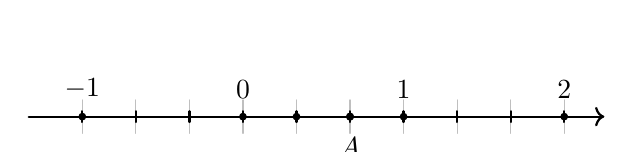
\begin{tikzpicture}[scale=0.85, line cap=round, line join=round]
    \draw[thick, ->] (-3.2, 0) -- (5.4, 0);
    \foreach \x in {-2.4, -1.6, -0.8, 0, 0.8, 1.6, 2.4, 3.2, 4.0, 4.8} {
        \draw[gray!50] (\x, -0.25) -- (\x, 0.25);
        \draw[thick] (\x, 0.08) -- (\x, -0.08);
    }
    \node[above=3pt] at (-2.4, 0) {$-1$};
    \node[above=3pt] at (0, 0) {$0$};
    \node[above=3pt] at (2.4, 0) {$1$};
    \node[above=3pt] at (4.8, 0) {$2$};
    \filldraw[black] (-2.4, 0) circle (1.4pt);
    \filldraw[black] (0, 0) circle (1.4pt);
    \filldraw[black] (0.8, 0) circle (1.4pt);
    \filldraw[black] (1.6, 0) circle (1.5pt) node[below=4pt, font=\bfseries] {$A$};
    \filldraw[black] (2.4, 0) circle (1.4pt);
    \filldraw[black] (4.8, 0) circle (1.4pt);
\end{tikzpicture}
}
\end{ex}

\begin{ex}
\immini{
Đọc tên các tia phân giác trong hình vẽ sau:
\choice
{$AB, BE$ là các tia phân giác}
{$AD, BC$ là các tia phân giác}
{\True $AD, BE$ là các tia phân giác}
{$AD, AB$ là các tia phân giác}
}{
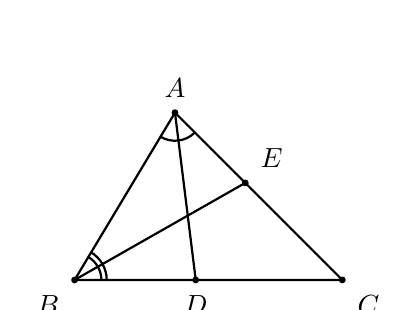
\begin{tikzpicture}[scale=0.85, line cap=round, line join=round]
    \coordinate (B) at (0, 0);
    \coordinate (C) at (4.0, 0);
    \coordinate (A) at (1.5, 2.5);
    \coordinate (D) at (1.81, 0);
    \coordinate (E) at (2.55, 1.45);

    \draw[thick] (A) -- (B) -- (C) -- cycle;
    \draw[thick] (A) -- (D);
    \draw[thick] (B) -- (E);

    \filldraw[black] (A) circle (1.2pt) node[above=2pt] {$A$};
    \filldraw[black] (B) circle (1.2pt) node[below left=2pt] {$B$};
    \filldraw[black] (C) circle (1.2pt) node[below right=2pt] {$C$};
    \filldraw[black] (D) circle (1.2pt) node[below=2pt] {$D$};
    \filldraw[black] (E) circle (1.2pt) node[above right=2pt] {$E$};

    % Bisector arcs at A
    \draw[thick] (A) ++(-121:0.42) arc (-121:-83:0.42);
    \draw[thick] (A) ++(-83:0.42) arc (-83:-45:0.42);
    % Bisector arcs at B
    \draw[thick] (B) ++(0:0.4) arc (0:29.5:0.4);
    \draw[thick] (B) ++(0:0.48) arc (0:29.5:0.48);
    \draw[thick] (B) ++(29.5:0.4) arc (29.5:59:0.4);
    \draw[thick] (B) ++(29.5:0.48) arc (29.5:59:0.48);
\end{tikzpicture}
}
\end{ex}

\begin{ex}
Hình nào dưới đây là hình lăng trụ đứng tam giác?
\choice
{\True Hình có hai đáy là tam giác và ba mặt bên là hình chữ nhật}
{Hình có hai đáy là tứ giác và bốn mặt bên là hình chữ nhật}
{Hình có hai đáy là hình vuông và bốn mặt bên là hình vuông}
{Hình có một đáy là tam giác, một đỉnh chung}
\end{ex}

\begin{ex}
Kết quả của phép tính $\left(-\dfrac{2}{5}\right)^2$ là:
\choice
{$-\dfrac{4}{25}$}
{\True $\dfrac{4}{25}$}
{$-\dfrac{2}{5}$}
{$\dfrac{4}{10}$}
\end{ex}

\begin{ex}
Số có thể viết dưới dạng số thập phân vô hạn tuần hoàn là:
\choice
{$\dfrac{3}{24}$}
{$-\dfrac{6}{25}$}
{\True $\dfrac{2}{15}$}
{$\dfrac{-5}{-8}$}
\end{ex}

\begin{ex}
Giá trị của $x$ thỏa mãn $|x| = 3$ là:
\choice
{$x = 3$}
{$x = -3$}
{\True $x = 3$ hoặc $x = -3$}
{$x = 9$}
\end{ex}

\begin{ex}
\immini{
Cho hình vẽ bên, cần thêm điều kiện gì thì $AB \parallel DC$?
\choice
{$\widehat{BCD} = 60^\circ$}
{$\widehat{BCD} = 120^\circ$}
{$\widehat{BAD} = 60^\circ$}
{\True $\widehat{xAB} = 60^\circ$}
}{
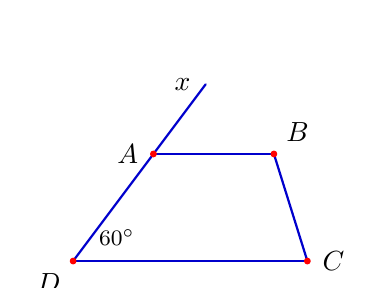
\begin{tikzpicture}[scale=0.85, line cap=round, line join=round]
    \coordinate (D) at (0, 0);
    \coordinate (C) at (3.5, 0);
    \coordinate (A) at (1.2, 1.6);
    \coordinate (B) at (3.0, 1.6);
    \coordinate (x) at ($(D)!1.65!(A)$);

    \draw[thick, blue!80!black] (D) -- (C);
    \draw[thick, blue!80!black] (A) -- (B);
    \draw[thick, blue!80!black] (B) -- (C);
    \draw[thick, blue!80!black] (D) -- (x);

    \filldraw[red] (A) circle (1.2pt) node[left=2pt, black] {$A$};
    \filldraw[red] (B) circle (1.2pt) node[above right=1pt, black] {$B$};
    \filldraw[red] (C) circle (1.2pt) node[right=2pt, black] {$C$};
    \filldraw[red] (D) circle (1.2pt) node[below left=1pt, black] {$D$};
    \node[left=2pt] at (x) {$x$};

    \node[font=\footnotesize, above right=1pt] at ($(D)+(0.2, 0.05)$) {$60^\circ$};
\end{tikzpicture}
}
\end{ex}

\newpage
\begin{ex}
Hãy so sánh hai số hữu tỉ $-0{,}2$ và $\dfrac{-2}{5}$:
\choice
{$-0{,}2 < \dfrac{-2}{5}$}
{\True $-0{,}2 > \dfrac{-2}{5}$}
{$-0{,}2 = \dfrac{-2}{5}$}
{$-0{,}2 \ge \dfrac{-2}{5}$}
\end{ex}

\begin{ex}
Căn bậc hai số học của $49$ là:
\choice
{$-7$}
{\True $7$}
{$-7$ và $7$}
{$-49$}
\end{ex}

\begin{ex}
Qua một điểm $M$ nằm ngoài đường thẳng $a$, kẻ được bao nhiêu đường thẳng song song với đường thẳng $a$?
\choice
{Có vô số đường thẳng}
{Không có đường thẳng nào}
{Có hai đường thẳng}
{\True Chỉ có một đường thẳng}
\end{ex}

\begin{ex}
Kết quả của phép tính $\dfrac{-3}{20} + \dfrac{-2}{15}$ là:
\choice
{$-\dfrac{1}{35}$}
{\True $-\dfrac{17}{60}$}
{$-\dfrac{5}{35}$}
{$-\dfrac{1}{60}$}
\end{ex}


\vspace{1mm}
\noindent\textbf{BẢNG TRẢ LỜI TRẮC NGHIỆM PHẦN I:}
\begin{center}
\begin{tabular}{|c|c|c|c|c|c|c|c|c|c|c|c|c|}
\hline
\textbf{Câu} & \textbf{1} & \textbf{2} & \textbf{3} & \textbf{4} & \textbf{5} & \textbf{6} & \textbf{7} & \textbf{8} & \textbf{9} & \textbf{10} & \textbf{11} & \textbf{12} \\
\hline
\textbf{Chọn} & \rule{0pt}{0.55cm} & & & & & & & & & & & \\
\hline
\end{tabular}
\end{center}
\vspace{1mm}

\setcounter{ex}{0}
\noindent\textbf{\large PHẦN II. CÂU TRẮC NGHIỆM ĐÚNG SAI (2,0 điểm)}

\textit{Thí sinh trả lời câu 1 và câu 2. Trong mỗi ý a), b), c), d) ở mỗi câu, thí sinh chọn đúng hoặc sai.}

\vspace{1mm}
\begin{ex}
Cho biểu thức $A = \left(-\dfrac{1}{2}\right)^3 + \dfrac{3}{4} \cdot \left(-\dfrac{2}{3}\right) + \left|-\dfrac{5}{8}\right|$. Xét tính đúng sai của các mệnh đề sau:
\choiceTF
{\True Giá trị của lũy thừa $\left(-\dfrac{1}{2}\right)^3$ bằng $-\dfrac{1}{8}$}
{\True Giá trị của phép tính $\dfrac{3}{4} \cdot \left(-\dfrac{2}{3}\right)$ bằng $-\dfrac{1}{2}$}
{Giá trị tuyệt đối $\left|-\dfrac{5}{8}\right|$ bằng $-\dfrac{5}{8}$}
{\True Giá trị của biểu thức $A$ bằng $0$}
\end{ex}

\begin{ex}
\immini{
Quan sát hình vẽ bên, hai đường thẳng $xx'$ và $yy'$ cắt nhau tại điểm $O$. Biết số đo góc $\widehat{xOy} = 45^\circ$. Xét tính đúng sai của các mệnh đề sau:
\choiceTF
{\True Góc $\widehat{xOy}$ và góc $\widehat{x'Oy'}$ là hai góc đối đỉnh}
{\True Số đo của góc $\widehat{x'Oy'}$ bằng $45^\circ$}
{\True Góc $\widehat{xOy'}$ kề bù với góc $\widehat{xOy}$ và có số đo bằng $135^\circ$}
{Tổng số đo của hai góc đối đỉnh $\widehat{xOy}$ và $\widehat{x'Oy'}$ bằng $180^\circ$}
}{
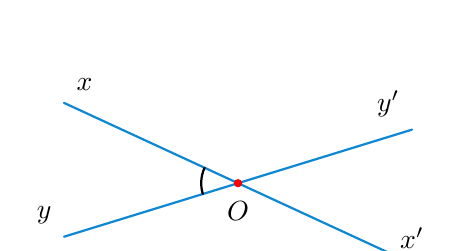
\begin{tikzpicture}[scale=0.85, line cap=round, line join=round]
    \coordinate (O) at (0, 0);
    \coordinate (x) at (-2.6, 1.2);
    \coordinate (x_prime) at (2.6, -1.2);
    \coordinate (y) at (-2.6, -0.8);
    \coordinate (y_prime) at (2.6, 0.8);

    \draw[thick, cyan!70!blue] (x) -- (x_prime);
    \draw[thick, cyan!70!blue] (y) -- (y_prime);

    \filldraw[red] (O) circle (1.5pt) node[below=3pt, black] {$O$};
    \node[above right=1pt] at (x) {$x$};
    \node[above=2pt] at (x_prime) {$x'$};
    \node[above left=1pt] at (y) {$y$};
    \node[above left=1pt] at (y_prime) {$y'$};

    % Arc for xOy
    \draw[thick] (O) ++(155.3:0.55) arc (155.3:197.1:0.55);
\end{tikzpicture}
}
\end{ex}


\noindent\textbf{BẢNG TRẢ LỜI PHẦN II:}
\begin{center}
\begin{tabular}{|c|c|c|c|c||c|c|c|c|c|}
\hline
\textbf{Câu 1} & \textbf{a)} & \textbf{b)} & \textbf{c)} & \textbf{d)} & \textbf{Câu 2} & \textbf{a)} & \textbf{b)} & \textbf{c)} & \textbf{d)} \\
\hline
\textbf{Đ/S} & \rule{0pt}{0.5cm} & & & & \textbf{Đ/S} & & & & \\
\hline
\end{tabular}
\end{center}
\vspace{1mm}

\setcounter{ex}{0}
\noindent\textbf{\large PHẦN III. CÂU HỎI TRẢ LỜI NGẮN (1,0 điểm)}

\textit{Thí sinh trả lời câu 1 và câu 2. Điền kết quả vào ô trống.}

\vspace{1mm}
\begin{ex}
Tìm số hữu tỉ $x$, biết: $\left(x - \dfrac{3}{4}\right)^2 = \dfrac{1}{16}$. \shortans{$x = 1$ hoặc $x = \dfrac{1}{2}$}
\end{ex}

\begin{ex}
Cho góc $\widehat{mOn} = 140^\circ$, tia $Ot$ là tia phân giác của $\widehat{mOn}$. Tính số đo góc kề bù với góc $\widehat{mOt}$. \shortans{$110^\circ$}
\end{ex}


\newpage
\setcounter{ex}{0}
\noindent\textbf{\large PHẦN IV. TỰ LUẬN (4,0 điểm)}

\textit{Thí sinh trình bày chi tiết lời giải vào giấy làm bài.}

\vspace{1mm}
\begin{ex}
Thực hiện phép tính:
\begin{enumerate}[label=\textbf{\alph*)}, leftmargin=0.8cm, itemsep=1pt]
\item $\dfrac{5}{12} + \left(-\dfrac{7}{24}\right) : \dfrac{3}{8}$;
\item $\dfrac{4}{5} \cdot \dfrac{3}{7} - \dfrac{-4}{7} : \sqrt{\dfrac{25}{16}} - |-1|$.
\end{enumerate}
\end{ex}
\vspace{2mm}

\begin{ex}
Tìm $x$ biết:
\begin{enumerate}[label=\textbf{\alph*)}, leftmargin=0.8cm, itemsep=1pt]
\item $2x - \dfrac{1}{3} = \dfrac{5}{3}$;
\item $(2x + 3)^2 = 25$.
\end{enumerate}
\end{ex}
\vspace{2mm}

\begin{ex}
Một hồ bơi dạng hình hộp chữ nhật có kích thước là chiều dài $12\text{ m}$, chiều rộng $5\text{ m}$ và chiều sâu $3\text{ m}$.
\begin{enumerate}[label=\textbf{\alph*)}, leftmargin=0.8cm, itemsep=1pt]
\item Tính thể tích nước khi bể bơi đầy nước.
\item Người ta cần lát gạch bên trong lòng hồ (mặt đáy và bốn mặt xung quanh). Biết gạch hình vuông có cạnh $50\text{ cm}$. Hỏi cần mua ít nhất bao nhiêu viên gạch để lát bên trong lòng hồ bơi? (Coi diện tích mạch vữa lát không đáng kể).
\end{enumerate}
\end{ex}
\vspace{2mm}

\begin{ex}
Cho $A = \dfrac{1}{2^2} + \dfrac{1}{3^2} + \dfrac{1}{3^4} + \dfrac{1}{3^6} + \ldots + \dfrac{1}{3^{100}}$. Chứng minh rằng $A < \dfrac{3}{8}$.
\end{ex}
\vspace{2mm}


\begin{center}
\rule{4cm}{0.4pt}\\
\textit{--- HẾT ---}
\end{center}
\end{document}
